\lecture{2}{20. Marts 2026}{Mathematical Models of Systems}

\subsection{Block Diagrams}
Though mathematical models are useful in describing the complex behavior of a control system they are often rather unintuitive.
A more graphical alternative to the rigorous mathematical models are Block Diagrams. An example of one of these is shown on \Cref{fig:block_diag_ex}

\begin{definition}[Block Diagram]
  A \textit{Block Diagram} is a schematic representation of the cause-and-effect relationshop throughout the system together with the transfer functions of the variables of interest.
\end{definition}

Typical elements of block diagrams include but are not limited to:
\begin{itemize}
  \item Comparators
  \item Blocks representing individual component transfer functions (sensors, actuators, controllers, plants, etc.)
  \item Input or reference signals
  \item Output signals
  \item Disturbance signals
  \item Feedback loops
\end{itemize}

\begin{figure} [ht]
  \centering
  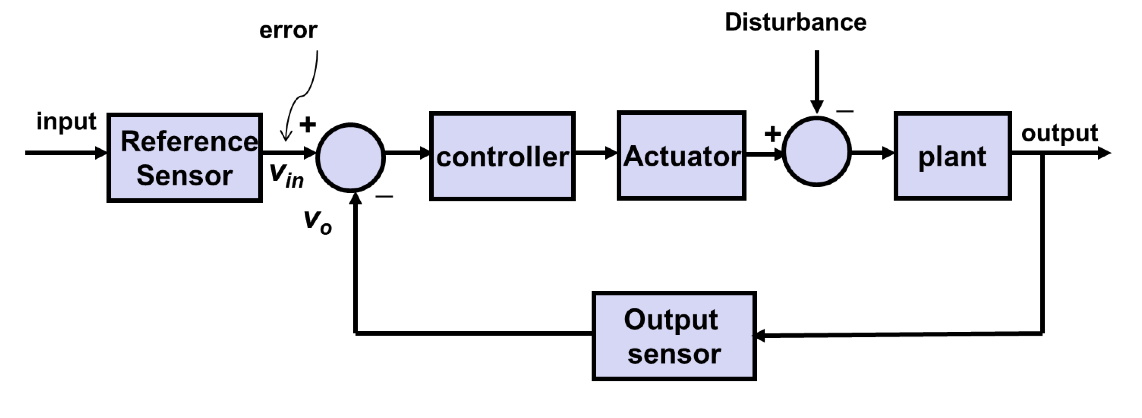
\includegraphics[width=0.65\linewidth]{./figures/block_diag_ex.png}
  \caption{Example of a block diagram.}
  \label{fig:block_diag_ex}
\end{figure}

An example showing how different components of a system might be represented as blocks of a block diagram is shown in \Cref{fig:block}.

\begin{figure} [ht]
  \centering
  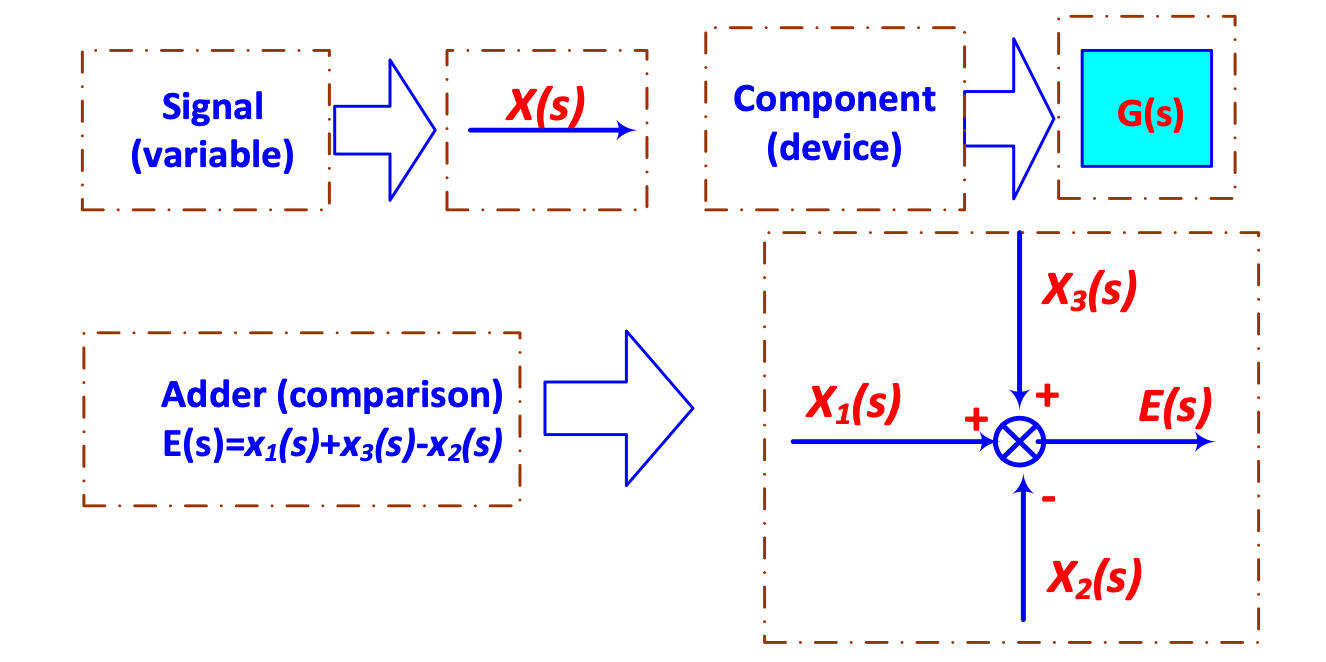
\includegraphics[width=0.5\linewidth]{./figures/block.png}
  \caption{Different components represented as blocks.}
  \label{fig:block}
\end{figure}

For multiple input or output systems the subscript convention is such that $G_{ij}$ is the transfer function of output $i$ and input $j$.

\subsubsection{Transformation and Reduction of Block Diagrams}
Different Block diagrams can be transformed and reduced into more simple forms.
This is especially useful for large and complex systems.

For a simple cascade block diagram as shown on \Cref{fig:casc} one is able to reduce the block diagram into a single $G_1 \cdot G_2$-block.
\begin{figure} [ht]
  \centering
  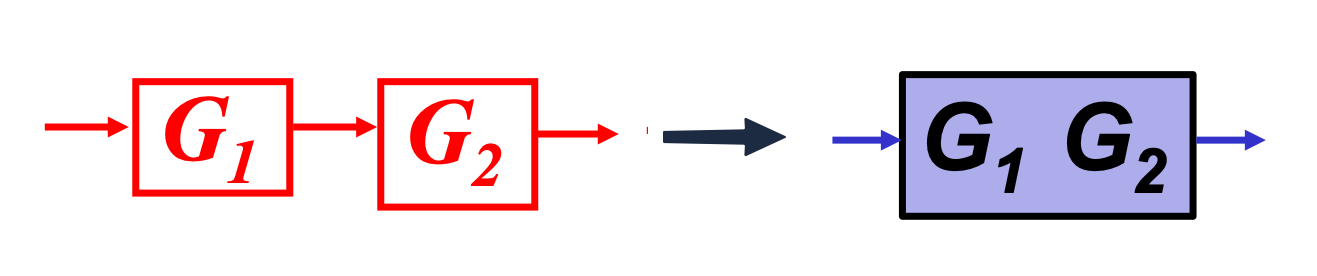
\includegraphics[width=0.5\linewidth]{./figures/casc.png}
  \caption{Cascade Block diagram.}
  \label{fig:casc}
\end{figure}

For a parallel block diagram as shown on \Cref{fig:parr} the resulting transformation is a single $G_1 - G_2$-block.
\begin{figure} [ht]
  \centering
  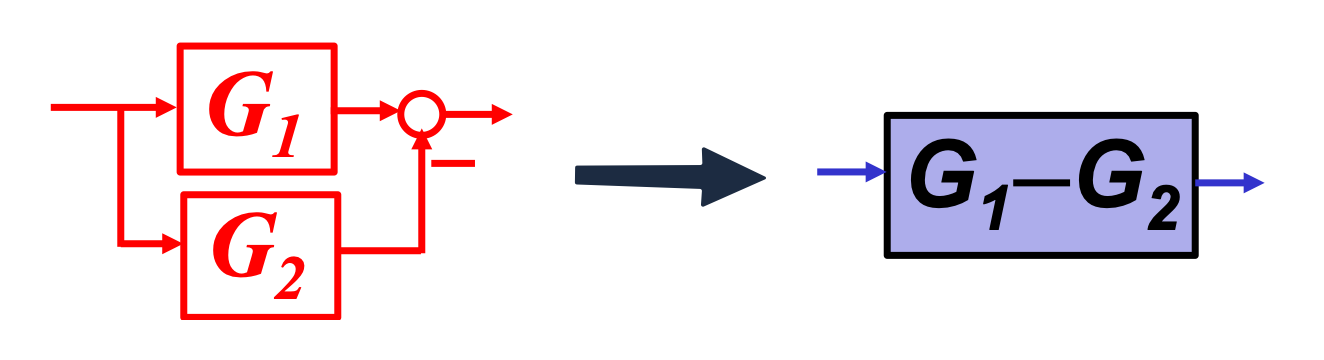
\includegraphics[width=0.5\linewidth]{./figures/parr.png}
  \caption{Parallel block diagram.}
  \label{fig:parr}
\end{figure}

For a negative feedback Block diagram as shown on \Cref{fig:feed} the reduction is a single block:
\begin{equation*}
  \frac{G_1}{1 + G_1 G_2}
.\end{equation*}
\begin{figure} [ht]
  \centering
  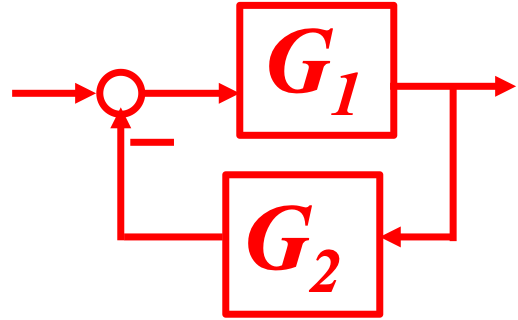
\includegraphics[width=0.3\linewidth]{./figures/feed.png}
  \caption{Feedback block diagram.}
  \label{fig:feed}
\end{figure}

\clearpage

A summing node is able to be moved across a block as shown in \Cref{fig:movnode}.
\begin{figure} [ht]
  \centering
  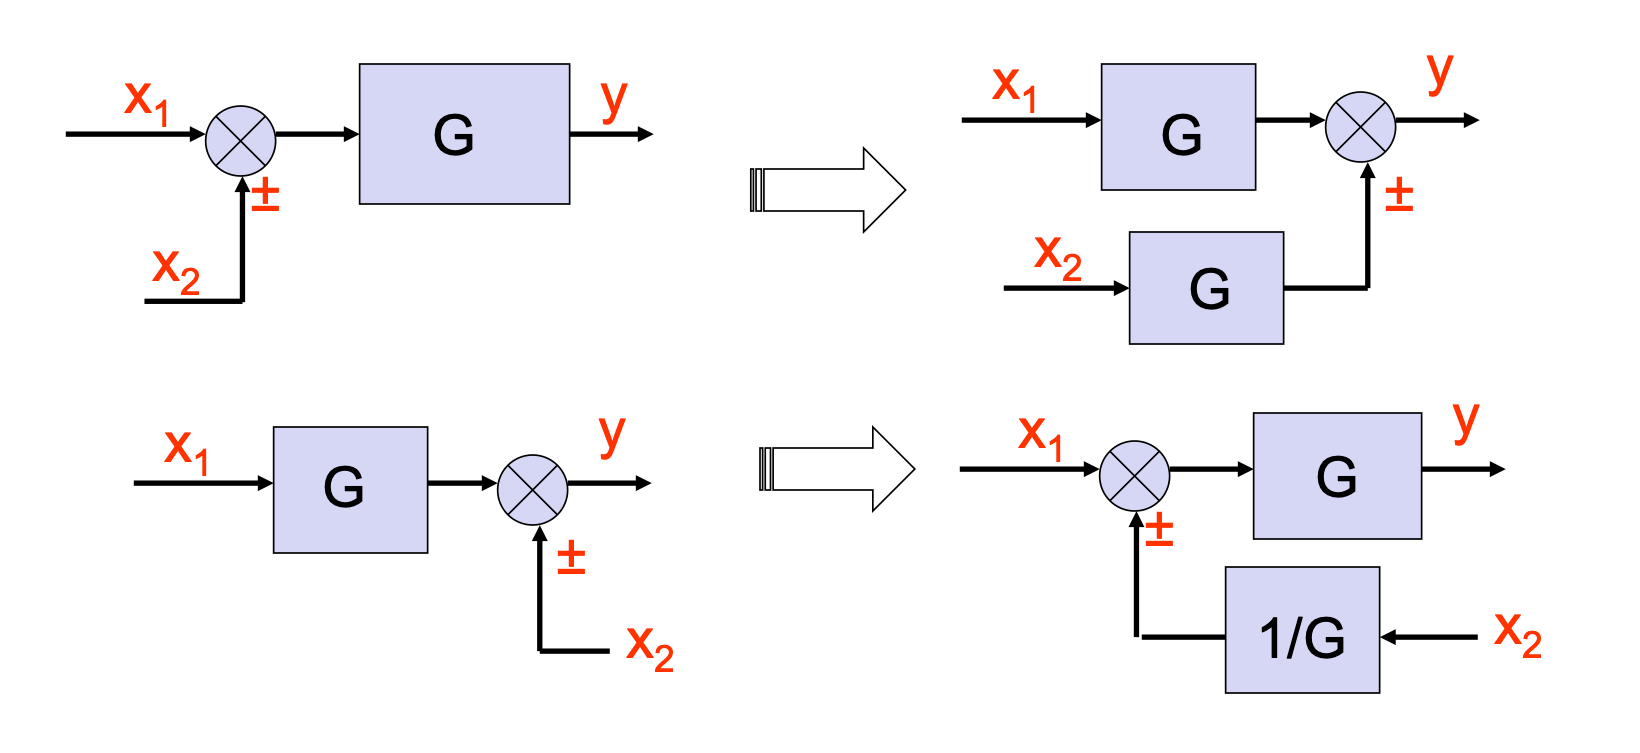
\includegraphics[width=0.65\linewidth]{./figures/movnode.png}
  \caption{Movement of a summing node across a block.}
  \label{fig:movnode}
\end{figure}

Pickoff points can also be moved across blocks.
The manner this is done by is shown in \Cref{fig:movpick}.

\begin{figure} [ht]
  \centering
  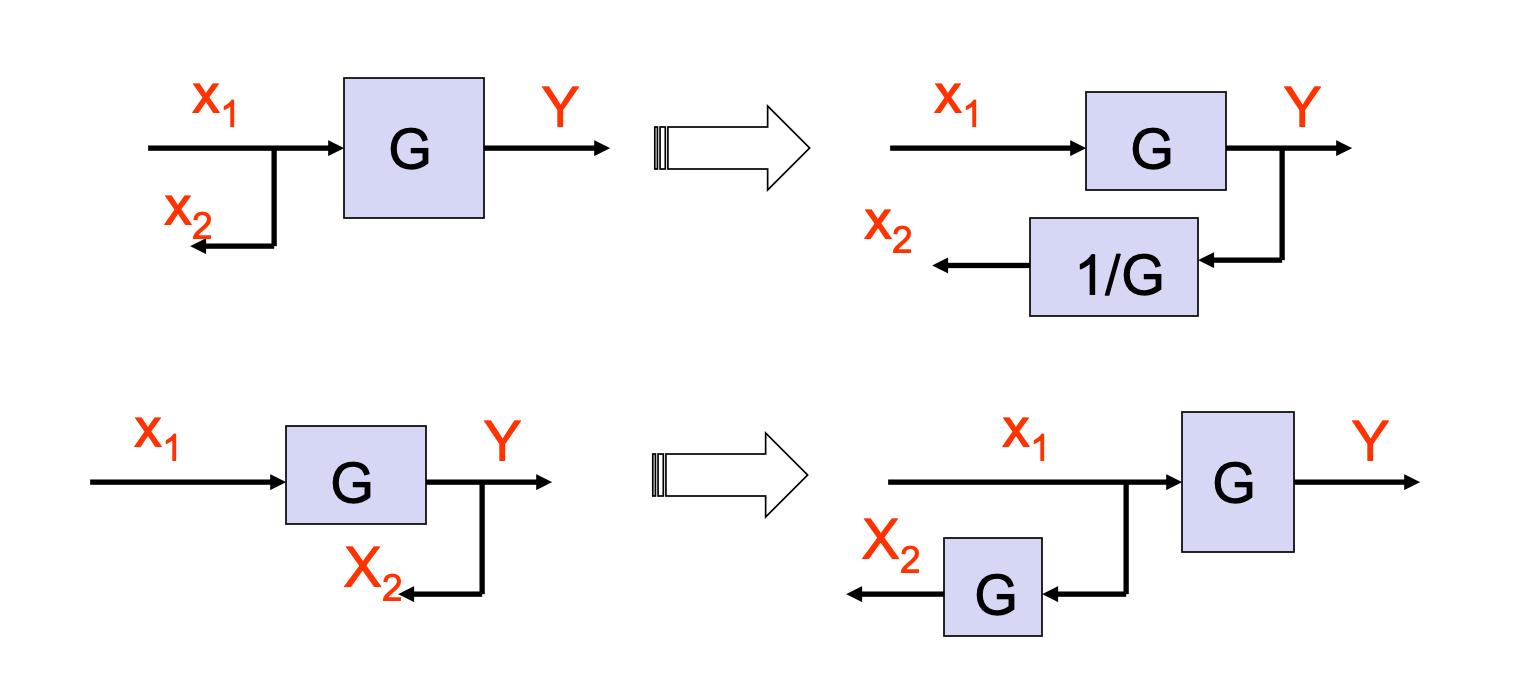
\includegraphics[width=0.65\linewidth]{./figures/movpick.png}
  \caption{Movement of a pickoff point across a block.}
  \label{fig:movpick}
\end{figure}

It is also possible to interchange neighboring summing points or pickoff points as shown in \Cref{fig:inter}.

\begin{figure} [ht]
  \centering
  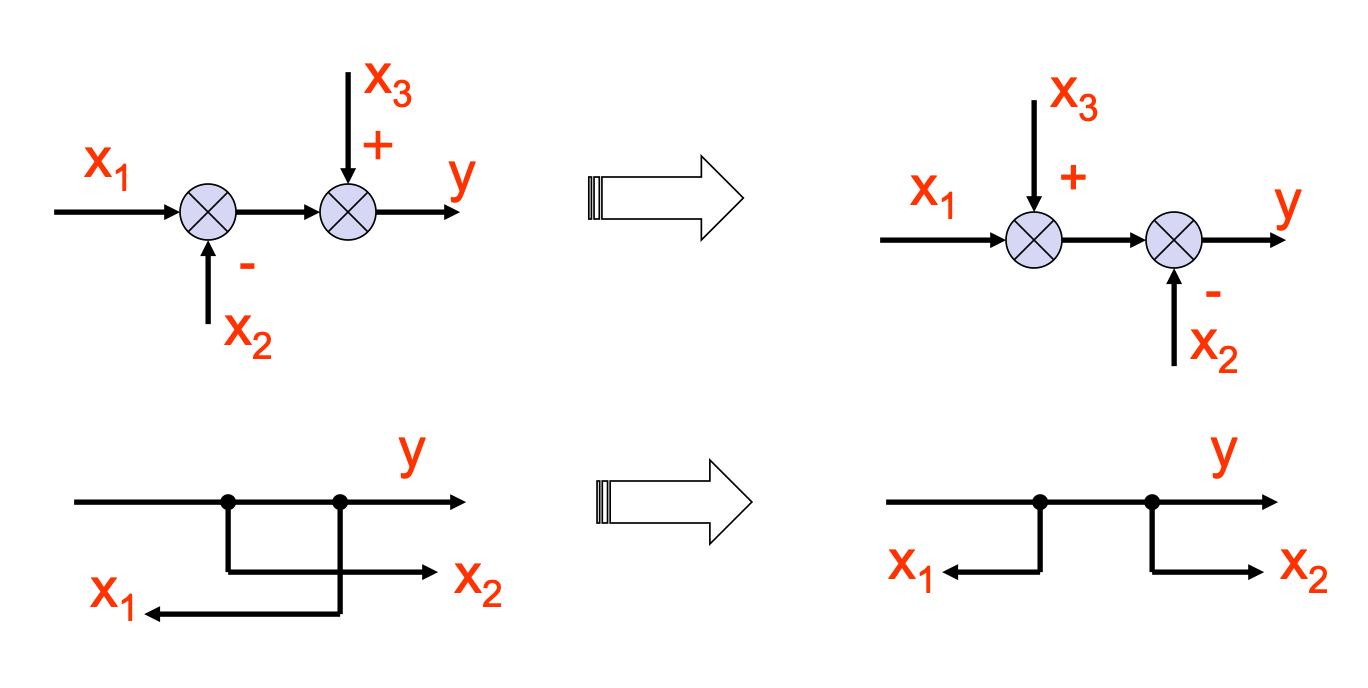
\includegraphics[width=0.65\linewidth]{./figures/inter.png}
  \caption{Interchanging neighboring summing and pickoff points}
  \label{fig:inter}
\end{figure}

\begin{exa}[Transfer function of an interacting system]
  Given the system shown find the transfer function.
  \tcblower
  We combine all the feedback loops using:
  \begin{equation*}
    G_i(s) || H_i(s) = \frac{G_i(s)}{1-G_i(s) H_i(s)}
  .\end{equation*}
  This gives:
  \begin{align*}
    G_2(s) || H_2(s) &= \frac{G_2(s)}{1 - G_2(s) H_2(s)} \\
    G_3(s) || H_3(s) &= \frac{G_3(s)}{1 - G_3(s) H_3(s)} \\
    G_6(s) || H_6(s) &= \frac{G_6(s)}{1 - G_6(s) H_6(s)} \\
    G_7(s) || H_7(s) &= \frac{G_7(s)}{1 - G_7(s) H_7(s)}
  .\end{align*}
  Now the two branches are both cascading, so using $G_1 G_2$ for series we get:
  \begin{align*}
    B_1(s) &= G_1(s) \cdot \frac{G_2(s)}{1 - G_2(s) H_2(s)} \cdot \frac{G_3(s)}{1 - G_3(s) H_3(s)} \cdot G_4(s) \\
    B_2(s) &= G_5(s) \cdot \frac{G_6(s)}{1 - G_6(s) H_6(s)} \cdot \frac{G_7(s)}{1 - G_7(s) H_7(s)} \cdot G_8(s)
  .\end{align*}
  Now, we are left with the two parallel $B_1(s)$ and $B_2(s)$ branches which are combined using $G_1 || G_2 = G_1 + G_2$ as:
  \begin{equation*}
    B_1(s) + B_2(s) = G_1(s) \cdot \frac{G_2(s)}{1 - G_2(s) H_2(s)} \cdot \frac{G_3(s)}{1 - G_3(s) H_3(s)} \cdot G_4(s) + G_5(s) \cdot \frac{G_6(s)}{1 - G_6(s) H_6(s)} \cdot \frac{G_7(s)}{1 - G_7(s) H_7(s)} \cdot G_8(s)
  .\end{equation*}
  Our transfer function is therefore:
  \begin{equation*}
    t(s) = G_1(s) \cdot \frac{G_2(s)}{1 - G_2(s) H_2(s)} \cdot \frac{G_3(s)}{1 - G_3(s) H_3(s)} \cdot G_4(s) + G_5(s) \cdot \frac{G_6(s)}{1 - G_6(s) H_6(s)} \cdot \frac{G_7(s)}{1 - G_7(s) H_7(s)} \cdot G_8(s)
  .\end{equation*}
  So
  \begin{equation*}
    Y(s) = R(s) \left(  G_1(s) \cdot \frac{G_2(s)}{1 - G_2(s) H_2(s)} \cdot \frac{G_3(s)}{1 - G_3(s) H_3(s)} \cdot G_4(s) + G_5(s) \cdot \frac{G_6(s)}{1 - G_6(s) H_6(s)} \cdot \frac{G_7(s)}{1 - G_7(s) H_7(s)} \cdot G_8(s) \right)
  \end{equation*}
  
\end{exa}
